\begin{title}
  Системы дифференциальных уравнений
\end{title}

\begin{title}[\Large]
  Системы обыкновенных дифференциальных уравнений. Векторная запись.
  Задача Коши
\end{title}

\begin{define}[системы обыкновенных дифференциальных уравнений]
  Запись в нормальной форме означает что в правой части нет производной
  $$
  \left\{
  \begin{array}{l}
    x_1'(t) = f_1(t, x_1(t), x_2(t), \ldots, x_n(t)) \\
    x_2'(t) = f_2(t, x_1(t), x_2(t), \ldots, x_n(t)) \\
    \ldots ~~~ \ldots ~~~ \ldots ~~~ \ldots ~~~ \ldots ~~~ \ldots \\
    x_n'(t) = f_n(t, x_1(t), x_2(t), \ldots, x_n(t))
  \end{array}
  \right.
  $$
  $$
  x(t) =
  \left(
  \begin{array}{l}
    x_1(t) \\
    x_2(t) \\
    \ldots \\
    x_n(t)
  \end{array}
  \right) ~~~
  f(t, x(t)) =
  \left(
  \begin{array}{l}
    f_1(t, x_1(t), x_2(t), \ldots, x_n(t)) \\
    f_2(t, x_1(t), x_2(t), \ldots, x_n(t)) \\
    \ldots ~~~ \ldots ~~~ \ldots ~~~ \ldots ~~~ \ldots \\
    f_n(t, x_1(t), x_2(t), \ldots, x_n(t))
  \end{array}
  \right)
  $$
  $x'(t) = f(t, x(t))$ где $x(t)$ неизвестный вектор функции
  $$
  x(t):<\alpha, \beta> \to R^n
  $$
  $$
  f(t, n): <\alpha, \beta> \times R^n \to R^n
  $$
\end{define}

\begin{block}[Задача Коши]
  $$
  t_0 \in <\alpha, \beta> ~~~ x_0 \in R^n ~~~
  \left\{
  \begin{array}{l}
    x'(t) = f(t,x(t)) \\
    x(t_0) = x_0
  \end{array}
  \right.
  $$
\end{block}

\begin{block}[Решением системы CОДУ называется]
  $\varphi(t): ~ <\alpha, \beta> \to R^n$

  1) непрерывна дифференциируема на $<\alpha, \beta>$

  2) $\forall t \in <\alpha, \beta> ~~~ (t, \varphi(t)) \in D$

  3) $\forall t \in <\alpha, \beta> ~~~ \frac{d\varphi(t)}{dt} \equiv
  f(t, \varphi(t))$
\end{block}

\begin{title}[\Large]
  Системы линейных дифференциальных уравнений в нормальной форме,
  матрично-векторная запись. Эквивалентность комплексной и вещественной системы
\end{title}

\begin{define}[системы линейных дифференциальных урвнений в нормальной форме]
  $$
  \left\{
  \begin{array}{l}
    x'_1(t) = a_{11}(t)x_1(t) + a_{12}(t)x_2(t) + \ldots
    + a_{1n}x_n(t) + g_1(t) \\
    x'_2(t) = a_{21}(t)x_1(t) + a_{22}(t)x_2(t) + \ldots
    + a_{2n}x_n(t) + g_2(t) \\
    \ldots ~~~ \ldots ~~~ \ldots ~~~ \ldots ~~~ \ldots ~~~ \ldots ~~~
    \ldots ~~~ \ldots ~~~ \ldots ~~~ \ldots\\
    x'_n(t) = a_{n1}(t)x_1(t) + a_{n2}(t)x_2(t) + \ldots
    + a_{nn}x_n(t) + g_n(t) \\
  \end{array}
  \right.
  $$
  $$
  x(t) =
  \left(
  \begin{array}{l}
    x_1(t) \\
    x_2(t) \\
    \ldots \\
    x_n(t)
  \end{array}
  \right) ~~~
  A(t) =
  \left(
  \begin{array}{cccc}
    a_{11}(t) & a_{12}(t) & \ldots & a_{1n}(t) \\
    a_{21}(t) & a_{22}(t) & \ldots & a_{2n}(t) \\
    \ldots & \ldots & \ldots & \ldots \\
    a_{n1}(t) & a_{n2}(t) & \ldots & a_{nn}(t)
  \end{array}
  \right) ~~~
  g(t) =
  \left(
  \begin{array}{l}
    g_1(t) \\
    g_2(t) \\
    \ldots \\
    g_n(t) \\
  \end{array}
  \right)
  $$
  $x'(t) = A(t)x(t) + g(t)$ неоднородная система линейных ДУ в нормальной форме

  $x'(t) = A(t)x(t)$ однородная система линейных ДУ в нормальной форме
\end{define}

\begin{block}[Эквивалентность комплексной и вещественной системы]
  $a_{ij}(t), g(t)$ непрерывны на $<\alpha, \beta> \in \mathbb{C}^n$

  $A(t) = A_1(t) + iA_2(t)$

  $g(t) = g_1(t) + ig_2(t)$

  $x(t) = x_1(t) + ix_2(t)$
  $$
  x'(t) = A(t)x(t) + g(t)
  $$
  $$
  x'_1(t) + ix'_2(t) = (A_1(t) + iA_2(t)) (x_1(t) + ix_2(t)) +
  (g_1(t) + ig_2(t)) =
  $$
  $$
  = A_1(t)x_1(t) + iA_2(t)x_1(t) + iA_1(t)x_2(t) - A_2(t)x_2(t) +
  g_1(t) + ig_2(t)
  $$
  $$
  \left\{
  \begin{array}{l}
    x'_1(t) = A_1(t)x_1(t) - A_2(t)x_2(t) + g_1(t) \\
    ix'_2(t) = iA_2(t)x_1(t) + iA_1(t)x_2(t) + ig_2(t)
  \end{array}
  \right.
  $$
  $$
  \left\{
  \begin{array}{l}
    x'_1(t) = A_1(t)x_1(t) - A_2(t)x_2(t) + g_1(t) \\
    x'_2(t) = A_2(t)x_1(t) + A_1(t)x_2(t) + g_2(t)
  \end{array}
  \right.
  $$
  $$
  \left(
  \begin{array}{c}
    x_1'(t) \\
    x_2'(t)
  \end{array}
  \right) =
  \left(
  \begin{array}{cc}
    A_1(t) & -A_2(t) \\
    A_2(t) & A_1(t)
  \end{array}
  \right)
  \left(
  \begin{array}{c}
    x_1(t) \\
    x_2(t)
  \end{array}
  \right) +
  \left(
  \begin{array}{c}
    g_1(t) \\
    g_2(t)
  \end{array}
  \right)
  $$
\end{block}

\begin{title}[\Large]
  Лемма об эквивалентности задачи Коши для линейной системы интегральному
  уравнению
\end{title}

\begin{block}[Лемма об эквивалентности задачи Коши для линейной системы]
  Задача Коши эквивалентна
  $$
  x(t) = x_0 + \int_{t_0}^t A(s)x(s)ds +
  \int_{t_0}^t g(s)ds
  $$
  то есть любое решение задачи Коши явялется решением этого уравнения и наоборот.
\end{block}

\begin{proof}
  $\Rightarrow$ $\varphi(t)$ решение задачи Коши тогда
  $$
  \varphi'(t) = A(t)\varphi(t) + g(t)
  $$
  $$
  \int_{t_0}^t \varphi'(s)ds = \int_{t_0}^t A(s) \varphi(s)ds +
  \int_{t_0}^t g(s) ds
  $$
  $$
  \varphi(t) = x_0 + \int_{t_0}^t A(s) \varphi(s) ds  + \int_{t_0}^t g(s)ds
  $$
  $\Leftarrow$ $\varphi(t)$ решение
  $$
  \varphi(t) = x_0 + \int_{t_0}^t A(s)\varphi(s)dx +
  \int_{t_0}^t g(s)ds
  $$
  тогда $\varphi(t)$ непрерывная $\Rightarrow$ дифференцируема
\end{proof}

\begin{title}[\Large]
  Теорема о существовании и единственности решения задачи Коши для линейной
  системы (построение и сходимость последовательных приближений,
  единственность решения)
\end{title}

\begin{block}[Задача Коши для линейной системы ДУ]
  $$
  t_0 \in <\alpha, \beta> ~~~ x_0 \in R^n ~~~
  \left\{
  \begin{array}{l}
    x'(t) = A(t)x(t) + g(t) \\
    x(t_0) = x_0
  \end{array}
  \right.
  $$
  $\varphi(t) : ~ <a,b> \to R^n$ решение задачи Коши

  $\phi(t) : ~ <c,d> \to R^n$  решение задачи Коши

  если $<c,d> \subset<a,b>$ и $t \in <c,d> ~~ \varphi(t) \equiv \phi(t)$ тогда

  $\varphi(t)$ это {\bfseries продолжение} $\phi(t)$

  $\phi$ это {\bfseries часть} $\varphi(t)$

  Решение называется {\bfseries непродолжимым} если оно не является частью никакого
  другого решения.
\end{block}

\begin{theorem}
  $A(t), g(t)$ непрерывны на $<\alpha, \beta>$ тогда
  $\forall t_0 \in <\alpha, \beta> ~~ \forall x_0 \in R^n$ задача Коши
  $\exists !$ решение на $<\alpha, \beta>$
\end{theorem}

\begin{proof}
  1) Построим последовательные приближения
  $$
  \varphi_0(t_0) = x_0 ~~~ t \in <\alpha, \beta>
  $$
  $$
  \varphi_1(t) = x_0 + \int_{t_0}^t A(s) \varphi_0(s)ds + \int_{t_0}^t g(s) ds
  ~~~ t \in <\alpha, \beta>
  $$
  $$
  \varphi_2(t) = x_0 + \int_{t_0}^t A(s) \varphi_1(s)ds + \int_{t_0}^t g(s) ds
  ~~~ t \in <\alpha, \beta>
  $$
  $$
  \ldots ~~~~~~~ \ldots ~~~~~~~ \ldots ~~~~~~~ \ldots ~~~~~~~ \ldots
   ~~~~~~~ \ldots ~~~~~~~ \ldots
  $$
  $$
  \varphi_{k+1}(t) = x_0 + \int_{t_0}^t A(s) \varphi_k(s)ds +
  \int_{t_0}^t g(s)ds ~~~ t \in <\alpha, \beta>
  $$

  2) Докажем что $\{\varphi_k(t)\}$ сходится на $<\alpha, \beta>$ к
  $\varphi(t)$ которая является решением задачи Коши

  $[c,d] \in <\alpha, \beta>$
  $$
  L = \sup_{t \in [c,d]} ||A(t)|| ~~~ M = \sup_{t \in [c,d]} ||\varphi_1(t) -
  \varphi_0(t)||
  $$
  Вместо последовательности расмотрим ряд
  $$
  \varphi_0(t) + \sum_{j=0}^{\infty}(\varphi_{j+1}(t) - \varphi_j(t))
  $$
  $$
  ||\varphi_1(t) - \varphi_0(t)|| \le M
  $$
  $$
  ||\varphi_2(t) - \varphi_1(t)|| =
  $$
  $$
  = \left\Vert x_0 + \int_{t_0}^t A(s)\varphi_1(s)ds +
  \int_{t_0}^t g(s)ds - x_0 - \int_{t_0}^t A(s)\varphi_0(s)ds -
  \int_{t_0}^t g(s)ds\right\Vert =
  $$
  $$
  = \left\Vert \int_{t_0}^t A(s)(\varphi_1(s) - \varphi_0(s))ds\right\Vert \le
  $$
  $$
  \colorbox[rgb]{0.7,0.7,0}{$\left\Vert \int_{t_1}^{t_2} f(x)dx \right\Vert
  \le \left| \int_{t_1}^{t_2} \left\Vert f(x)\right\Vert dx \right|$}
  $$
  $$
  \le \left| \int_{t_0}^t \left\Vert A(s)(\varphi_1(s) - \varphi_0(s))
  \right\Vert ds \right| \le
  $$
  $$
  \le \left| \int_{t_0}^t \left\Vert A(s)\right\Vert
  \left\Vert (\varphi_1(s) - \varphi_0(s)) \right\Vert ds \right| \le
  $$
  $$
  \le ML \left| \int_{t_0}^{t} ds \right| = ML|t-t_0|
  $$
  $$
  ||\varphi_3(t) - \varphi_2(t)|| \le \left| L \int_{t_0}^t||\varphi_2(s) -
  \varphi_1(s)||ds \right| \le L^2 M \left| \int_{t_0}^t |s - t_0| ds \right| =
  $$
  $$
  t > t_0 ~~~ \left| \int_{t_0}^t |s - t_0| ds \right| = \frac{(t- t_0)^2}{2}
  $$
  $$
  t < t_0 ~~~ \left| \int_{t_0}^t |t_0 - s| ds \right| = \frac{(t- t_0)^2}{2}
  $$
  $$
  = L^2 M \frac{(t- t_0)^2}{2}
  $$
  $$
  ||\varphi_{k+1}(t) - \varphi_k(t)|| \le L^k M \frac{|t - t_0|^k}{k!}
  $$
  $$
  ||\varphi_{k+2}(t) - \varphi_{k+1}(t)|| \le \left| \int_{t_0}^t ||A(s)|| ~
  ||\varphi_{k+1}(s) - \varphi_k(s)|| ds \right| \le
  $$
  $$
  \le \frac{L^{k+1}M}{k!} \left| \int_{t_0}^t |s - t_0|^k ds \right| =
  \frac{L^{k+1}M|t-t_0|^{k+1}}{(k+1)!}
  $$
  $$
  \sum_{k=0}^{\infty} \frac{L^kM(d - c)^k}{k!}
  $$
  докажем сходимость по Доламберу
  $$
  \lim_{k \to \infty} \frac{L^{k+1} M(d - c)^{k+1}k!}{(k+1)!L^k M (d - c)^k} =
  \lim_{k \to \infty} \frac{L(d-c)}{k+1} = 0 < 1 ~ \Rightarrow ~
  \text{сходится}
  $$
  $\Rightarrow$ по признаку Вейерштраса
  $$
  \varphi_0(t) + \sum_{j=0}^{\infty}(\varphi_{j+1}(t) - \varphi_j(t))
  $$
  сходится равномерно на $[c,d]$

  $\lim_{k \to \infty} \varphi_k(t) = \varphi(t)$ непрерывна
  $$
  \varphi_{k+1} = x_0 + \int_{t_0}^t A(s) \varphi_k(s) ds + \int_{t_0}^t g(s)ds
  ~~~ k \to \infty
  $$
  $$
  \varphi = x_0 + \int_{t_0}^t A(s) \varphi(s) ds + \int_{t_0}^t g(s)ds
  $$
  по Лемме $\varphi(t)$ решение задачи Коши

  3) Докажем единственность решения задачи Коши
  $$
  \varphi = x_0 + \int_{t_0}^t A(s) \varphi(s) ds + \int_{t_0}^t g(s)ds
  $$
  $$
  \psi = x_0 + \int_{t_0}^t A(s) \psi(s) ds + \int_{t_0}^t g(s)ds
  $$
  $$
  N = \sup_{t \in [c,d]} ||\varphi(t) - \psi(t)||
  $$
  $$
  ||\varphi(t) - \psi(t)|| = \left\Vert\int_{t_0}^t A(s)
  (\varphi(s) - \psi(s))ds \right\Vert \le \left| \int_{t_0}^t ||A(s)|| ~
  ||\varphi(s) - \psi(s)||ds \right| \le
  $$
  $$
  \le LN|t-t_0| \le L^2 N \frac{(t - t_0)^2}{2} \le
  \frac{L^k M (t - t_0)^k}{k!} \to 0 ~~ k \to \infty
  $$
  $\Rightarrow$ $\varphi(t) \equiv \psi(t)$
\end{proof}

\begin{theorem}
  Всякое решение задачи Коши это часть непродолжимого решения.
\end{theorem}

\begin{title}[\Large]
  Линейные системы дифференциальных уравнений, принцип суперпозиции решений и
  следствия из него
\end{title}

\begin{theorem}[приципа суперпозии решений]
  $\varphi(t)$ решение $x'(t) = A(t)x(t) + g_1(t)$

  $\psi(t)$ решение $x'(t) = A(t)x(t) + g_2(t)$

  тогда $C\varphi(t) + B\psi(t)$ решение $x'(t) = A(t)x(t) + Cg_1(t) + Bg_2(t)$
  $C,B$ числа
\end{theorem}

\begin{proof}
  $$
  C\varphi'(t) + B\psi'(t) = A(t)(C\varphi(t) + B\psi(t)) + Cg_1(t) +
  Bg_2(t)
  $$
  $$
  C\varphi'(t) + B\psi'(t) =
  C \overbrace{(A(t)\varphi(t) + g_1(t))}^{\varphi'(t)}+
  B \overbrace{(A(t)\psi(t) + g_2(t))}^{\psi'(t)}
  $$
\end{proof}

\begin{block}[Следствие 1]
  Разность двух решений неоднородной линейной системы является решением
  однородной линейной системы.
\end{block}

\begin{proof}
  $x'(t) = A(t)x(t) + g(t) ~~ C = 1 ~~ B = 1$

  $\varphi(t) - \psi(t)$

  $g(t) - g(t) = 0$
\end{proof}

\begin{block}[Слeдствие 2]
  $\varphi_0(t)$ частное решение системы $x'(t) = A(t)x(t) + g(t)$ то
  множество всех решений этой системы совпадает с множеством следующего вида
  $\{\varphi_0(t) + \varphi(t)\}$ где $\varphi(t)$ множество решений
  $x'(t) = A(t)x(t)$
\end{block}

\begin{proof}
  $\varphi_0(t)$ решение $x'(t) = A(t)x(t) + g(t)$

  $\varphi(t)$ решение $x'(t) = A(t)x(t)$

  $\varphi_0(t) + \varphi(t)$ решение $x'(t) = A(t)x(t) + g(t)$

  Пусть $\psi(t)$ решение $x'(t) = A(t)x(t) + g(t)$

  $\psi(t) - \varphi_0(t)$ решение $x'(t) = A(t)x(t)$

  $\Rightarrow ~ \psi(t) = \varphi_0(t) - \varphi(t)$
\end{proof}

\begin{title}[\Large]
  Линейная зависимость и независимость вектор-функций
\end{title}

\begin{define}[вектор функции, ЛЗ и ЛНЗ]
  $$
  \varphi_1 (t) =
  \left(
  \begin{array}{c}
    \varphi_{11}(t) \\
    \cdots \\
    \varphi_{1n}(t) \\
  \end{array}
  \right),~~~
  \varphi_2 (t) =
  \left(
  \begin{array}{c}
    \varphi_{21}(t) \\
    \cdots \\
    \varphi_{2n}(t) \\
  \end{array}
  \right), \cdots,
  \varphi_k (t) =
  \left(
  \begin{array}{c}
    \varphi_{k1}(t) \\
    \cdots \\
    \varphi_{kn}(t) \\
  \end{array}
  \right) ~~~ t \in <\alpha, \beta>
  $$
  $\varphi, \cdots, \varphi_k(t)$ называется ЛЗ если $\exists C_1, C_2, \ldots,
  C_k ~~ \sum_{j=1}^k C_j^2 \not= 0 ~~ \forall t \in <\alpha, \beta> ~
  C_1\varphi_1(t) + C_2\varphi_2(t) + \ldots + C_k\varphi_k(t) = 0$. В
  противном случае система функций ЛНЗ.
\end{define}

\begin{title}[\Large]
  Линейные однородные системы. Пространство решений. Фундаментальная система
  решений
\end{title}

\begin{theorem}
  Множество всех решений $x'(t) = A(t)x(t)$ образует
  линейное пространство размерность которого совпадает с размерностью системы.
\end{theorem}

\begin{proof}
  1) Если $\varphi_1(t), \varphi_2(t)$ решение $x'(t) = A(t)x(t) ~ \Rightarrow ~
  C_1\varphi_1(t) + C_2\varphi_2(t)$ решение $x'(t) = A(t)x(t)$
  $$
  C_1 \varphi'_1(t) + C_2 \varphi'_2(t) = C_1A(t) \varphi_1(t) +
  C_2A(t)\varphi_2(t) = A(t)(C_1\varphi_1(t) + C_2\varphi_2(t)) ~ \Rightarrow
  $$
  $C_1 \varphi_1(t) + C_2 \varphi_2(t)$ решение $x'(t) = A(t)x(t)$\\

  2) Построим $n$ ЛНЗ решений на $<\alpha, \beta>$ и $t_0 \in <\alpha, \beta>$
  $$
  \varphi_1 =
  \left(
  \begin{array}{c}
    1 \\
    0 \\
    \cdots \\
    0
  \end{array}
  \right), ~~~
  \varphi_2 =
  \left(
  \begin{array}{c}
    0 \\
    1 \\
    \cdots \\
    0
  \end{array}
  \right), \cdots,
  \varphi_n =
  \left(
  \begin{array}{c}
    0 \\
    0 \\
    \cdots \\
    1
  \end{array}
  \right)
  $$
  $$
  \left\{
  \begin{array}{l}
    x'(t) = A(t)x(t) \\
    x(t_0) = \varphi_k
  \end{array}
  \right. ~~~ k = 1, 2, \ldots, n
  $$
  $\varphi_k(t)$ единственое решение

  покажем ЛНЗ $C_1 \varphi_1(t) + \ldots + C_n \varphi_n(t) \equiv 0$
  $$
  t = t_0 ~~~ C_1 \varphi_1(t_0) + C_2 \varphi_2(t_0) + \ldots +
  C_n \varphi_n(t_0) \equiv 0
  $$
  $$
  C_1
  \left(
  \begin{array}{c}
    1 \\
    0 \\
    \cdots \\
    0
  \end{array}
  \right) +
  C_2
  \left(
  \begin{array}{c}
    0 \\
    1 \\
    \cdots \\
    0
  \end{array}
  \right) + \cdots +
  C_n
  \left(
  \begin{array}{c}
    0 \\
    0 \\
    \cdots \\
    1
  \end{array}
  \right) =
  \left(
  \begin{array}{c}
    0 \\
    0 \\
    \cdots \\
    0
  \end{array}
  \right)
  $$
  $$
  \left(
  \begin{array}{c}
    C_1 \\
    C_2 \\
    \cdots \\
    C_n
  \end{array}
  \right) =
  \left(
  \begin{array}{c}
    0 \\
    0 \\
    \cdots \\
    0
  \end{array}
  \right) ~ \Rightarrow ~ C_1 = C_2 = \ldots = C_n = 0 ~ \Rightarrow ~
  \varphi_1(t), \ldots, \varphi_n(t) ~ \text{ЛНЗ}
  $$
  3) $\psi(t)$ произвольное решение
  $$
  \psi(t_0) =
  \left(
  \begin{array}{c}
    a_1 \\
    a_2 \\
    \cdots \\
    a_n
  \end{array}
  \right)
  $$
  $\varphi = a_1 \varphi_1(t) + \ldots + a_n \varphi_n(t)$

  Заменим:
  $$
  \psi(t) =
  \left\{
  \begin{array}{l}
  x'(t) = A(t)x(t)\\
  x(t_0) =
  \left(
  \begin{array}{c}
    a_1 \\
    a_2 \\
    \cdots \\
    a_n
  \end{array}
  \right)
  \end{array}
  \right. ~ \text{на} ~~~ \varphi(t) =
  \left\{
  \begin{array}{c}
  x'(t) = A(t)x(t)\\
  x(t_0) =
  \left(
  \begin{array}{c}
    a_1 \\
    a_2 \\
    \cdots \\
    a_n
  \end{array}
  \right)
  \end{array}
  \right.
  $$
  $$
  \varphi(t_0) = a_1 \varphi_1(t_0) + \ldots + a_n \varphi_n(t_0) =
  a_1
  \left(
  \begin{array}{c}
    1 \\
    0 \\
    \cdots \\
    0
  \end{array}
  \right) +
  a_2
  \left(
  \begin{array}{c}
    0 \\
    1 \\
    \cdots \\
    0
  \end{array}
  \right) + \ldots +
  a_n
  \left(
  \begin{array}{c}
    0 \\
    0 \\
    \cdots \\
    1
  \end{array}
  \right) =
  \left(
  \begin{array}{c}
    a_1 \\
    a_2 \\
    \cdots \\
    a_n
  \end{array}
  \right)
  $$
  так как они обе удовлетворяеют задачи Коши то $\varphi(t) \equiv \psi(t) ~
  \Rightarrow$
  $$
  \psi(t) = \sum_{j=1}^n a_j \varphi_j(t)
  $$
\end{proof}

\begin{define}[ФСР СЛДУ]
  ФСР называется базис пространства решений то есть $n$ ЛНЗ решений данной
  системы.
\end{define}

\begin{title}[\Large]
  Определитель Вронского. Критерий линейной независимости решений однородной
  системы
\end{title}

\begin{define}[определителя Вронского]
  $\varphi_1(t), \ldots, \varphi_n(t)$ вектор функции
  $$
  \varphi_j(t) =
  \left(
  \begin{array}{c}
    \varphi_{j1}(t) \\
    \varphi_{j2}(t) \\
    \cdots \\
    \varphi_{jn}(t)
  \end{array}
  \right) ~~~~~~
  W[\varphi_1, \ldots, \varphi_n](t) =
  \left|
  \begin{array}{cccc}
    \varphi_{11}(t) & \varphi_{21}(t) & \ldots & \varphi_{n1}(t) \\
    \varphi_{12}(t) & \varphi_{22}(t) & \ldots & \varphi_{n2}(t) \\
    \ldots & \ldots & \ldots & \ldots \\
    \varphi_{1n}(t) & \varphi_{2n}(t) & \ldots & \varphi_{nn}(t)
  \end{array}
  \right|
  $$
\end{define}

\begin{block}[Утверждения]
  1) $\varphi_1(t), \ldots, \varphi_n(t)$ ЛЗ $\Rightarrow W(t) \equiv 0$

  2) $W(t) \not\equiv 0 ~ \Rightarrow ~ \varphi_1(t), \ldots, \varphi_n(t)$ ЛНЗ
\end{block}

\begin{block}[Критерий ЛНЗ решений системы]
  $\varphi_1, \ldots, \varphi_n(t)$ решение задачи Коши тогда

  1) $\exists t_0 \in <\alpha, \beta> ~~ W(t_0) = 0$ тогда решение
  $\varphi_1(t), \ldots, \varphi_n(t)$ ЛЗ

  2) $\varphi_1, \ldots, \varphi_n(t)$ ЛНЗ тогда $\forall t \in <\alpha, \beta>
  ~~ W(t) \not= 0$
\end{block}

\begin{proof}
  1) $t_0 \in <\alpha, \beta> ~~ W(t_0) = 0 ~ \Rightarrow ~ \varphi_1(t_0),
  \ldots, \varphi_n(t_0)$ ЛЗ $~\Rightarrow~$ $\exists C_1, \ldots, C_n ~~~
  C_1 \varphi_1(t_0) + \ldots + C_n \varphi_n (t_0) = 0$

  $\varphi(t) = C_1\varphi_1(t) + \ldots + C_n \varphi_n(t)$
  $$
  \varphi(t) =
  \left\{
  \begin{array}{l}
    x'(t) = A(t)x(t) \\
    x(t_0) = 0
  \end{array}
  \right.
  $$
  $\psi \equiv 0$ другое решение $\Rightarrow ~ \varphi(t) = C_1 \varphi_1(t) +
  \ldots + C_n \varphi_n(t) \equiv 0 ~ \Rightarrow ~ \varphi_1, \ldots,
  \varphi_n$ ЛЗ \\
\end{proof}

\begin{theorem}
  $W(t)$ решение $\varphi_1(t), \ldots, \varphi_n(t)$ системы $x'(t) = A(t)x(t)$
  тогда $t \in <\alpha, \beta> ~~~ \frac{dW(t)}{dt} = (trA(t))W(t)$
  $$
  trA(t) = \sum_{j=1}^n a_{jj}(t)
  $$
\end{theorem}

\begin{block}[Формула Леовиля]
  $$
  W(t) = W(t_0)e^{\int_{t_0}^t tr A(s)ds}
  $$
  если $\exists t_1 ~~ W(t_1) = 0$ тогда $W(t) \equiv 0$
\end{block}

\begin{title}[\Large]
  Фундаментальная матрица, свойства. Общее решение линейной однородной системы
\end{title}

\begin{define}[матрицы решения однородной системы]
  Матрица $\Phi(t) ~ t \in <\alpha, \beta>$ называется решением системы
  $x'(t) = A(t)x(t)$ если столбцы матрицы являются решением системы.
\end{define}

\begin{define}[фундаментальной матрицы решений]
  Невырожденная матрица решений называется фундаментальной матрицей
  $|\Phi(t)| = W(t)$ столбцы ЛНЗ. Фундаментальная матрица это матрица столбцы
  которой образуют ФСР.
\end{define}

\begin{block}[Утверждение]
  $\Phi(t)$ является матрицей решений $\Leftrightarrow$ удовлетворяет
  матричной системе
  $$
  X'_{n \times n}(t) = A_{n \times n}(t) X_{n \times n}(t)
  $$
\end{block}

\begin{theorem}
  $\Phi(t)$ фундаментальная матрица $x'(t) = A(t)x(t)$
  тогда множество решений системы совпадает со множеством функций вида
  $\varphi(t) = \Phi(t)C$ где $C$ произвольный постоянный вектор из
  $\mathbb{C}^n$
\end{theorem}

\begin{proof}
  $\Rightarrow$ $\Phi(t)$ фундаментальная матрица и $\varphi_1(t), \ldots,
  \varphi_n(t)$ это ФСР

  $\Leftarrow$ $\Phi(t)C = (\varphi_1(t), \ldots, \varphi_n(t))C = C_1
  \varphi_1(t) + C_2 \varphi_2(t) + \ldots + C_n \varphi_n(t)$
\end{proof}

\begin{theorem}
  $\Phi(t)$ фундаментальная матрица $x'(t) = A(t)x(t)$ тогда множество всех
  фундаментальных матриц системы совпадает с множеством матриц следующего вида
  $\Psi(t) = \Phi(t)B ~~ \det B_{n \times n} \not= 0$
\end{theorem}

\begin{proof}
  $\Rightarrow$ так как $\Phi(t)$ фундаментальная матрица $det\Phi(t) \not= 0 ~~
  \forall t \in <\alpha, \beta> ~~ \Phi'(t) = A(t)\Phi(t)$
  $det\Psi(t) \not= 0$ невырожденная

  $\Phi'(t)B = A(t)(\Phi(t)B)$

  $(\Phi(t)B)' = A(t)(\Phi(t)B)$

  $\Psi'(t) = A(t)\Psi(t)$ где $\Psi$ фундаментальная матрица

  $\Leftarrow$ пусть $\Psi(t)$ фиксированная фундаментальная матрица

  $t_0 \in <\alpha, \beta> ~~ B = \Phi^{-1}(t_0) \Psi(t_0)$

  $\Psi(t) = \Phi(t) \Phi^{-1}(t_0) \Psi(t_0)$

  $t = t_0 ~~~ \Psi(t_0) = \Phi(t_0) \Phi^{-1}(t_0) \Psi(t_0)$
  $$
  \left\{
  \begin{array}{l}
    X'(t) = A(t)X(t) \\
    X(t_0) = \Psi(t_0)
  \end{array}
  \right. ~ \Rightarrow ~
  \Psi(t) = \Phi(t) \Phi^{-1}(t_0)\Psi(t_0)
  $$
  одна фундаментальная матрица вырожена через другую
\end{proof}

\begin{title}[\Large]
  Линейные неоднородные системы дифференциальных уравнений. Метод вариаций.
  Формула Коши
\end{title}

\begin{block}[Метод вариаций для линейных неоднородных CДУ]
  $A(t), g(t)$ непрерывны на $<\alpha, \beta>$

  $x(t) = \Phi(t) C$ общее решение $x'(t) = A(t)x(t)$
  $$
  C =
  \left(
  \begin{array}{c}
    C_1 \\
    C_2 \\
    \cdots \\
    C_n
  \end{array}
  \right) ~~~
  C(t) =
  \left(
  \begin{array}{c}
    C_1(t) \\
    C_2(t) \\
    \cdots \\
    C_n(t)
  \end{array}
  \right)
  $$
  $$
  x(t) = \Phi(t)C(t)
  $$
  $$
  x'(t) = \Phi'(t)C(t) + \Phi(t)C'(t)
  $$
  $$
  \Phi'(t)C(t) + \Phi(t)C'(t) = A(t)\Phi(t)C(t) + g(t)
  $$
  $$
  \Phi'(t) = A(t) \Phi(t)
  $$
  $$
  \Phi(t)C'(t) = g(t)
  $$
  $$
  C'(t) = \Phi^{-1}(t)g(t)
  $$
  $$
  C(t) = \int_{t_0}^t \Phi^{-1}(s)g(s)ds + D
  $$
  $$
  x(t) = \Phi(t)D + \Phi(t)\int_{t_0}^t\Phi^{-1}(s)g(s)ds
  $$
  формула общего решения линейной неоднородной системы дифференциальных
  уравнений.
\end{block}

\begin{block}[Формула Коши]
  $$
  \left\{
  \begin{array}{l}
    x'(t) = A(t)x(t) + g(t) \\
    x(t_0) = x_0
  \end{array}
  \right. ~~~ \text{задача Коши}
  $$
  $$
  x(t_0) = \Phi(t_0)D
  $$
  $$
  D = \Phi^{-1}(t_0)x(t_0) = \Phi^{-1}(t_0)x_0
  $$
  $$
  x(t) = \Phi(t) \Phi^{-1}(t_0)x_0 + \Phi(t)\int_{t_0}^t \Phi^{-1}(s)g(s)ds
  $$
\end{block}

\begin{theorem}
  $A(t), g(t)$ непрерывные на $<\alpha, \beta>$ тогда
  решение задачи Коши определяется формулой Коши.
\end{theorem}

\begin{define}[матрицы Коши]
  $$
  C(t,s) = \Phi(t)\Phi^{-1}(s) ~ \text{матрица Коши}
  $$
  $$
  x(t) = C(t, t_0)x_0 + \int_{t_0}^t C(t,s)g(s)ds
  $$
\end{define}

\begin{theorem}
  $C(t,s)$ не зависит от выбора фундаментальной матрицы.
\end{theorem}

\begin{proof}
  Пусть $\Psi(t)$ другая фундаментальная матрица $D(t,s) = \Psi(t)\Psi^{-1}(s)$
  тогда $\exists B$ невырожденая матрица
  $$
  \Psi(t) = \Phi(t)B
  $$
  $$
  \colorbox[rgb]{0.7,0.7,0}{$(A\cdot B)^{-1} = B^{-1} \cdot A^{-1}$}
  $$
  $$
  \Psi^{-1}(s) = B^{-1} \Phi^{-1}(s)
  $$
  $$
  \Psi(t) \Psi^{-1}(s) = \Phi(t) B B^{-1} \Phi^{-1}(s)
  $$
  $$
  \Psi(t) \Psi^{-1}(s) = \Phi(t) \Phi^{-1}(s)
  $$
  $$
  D(t, s) = C(t, s)
  $$
\end{proof}

\begin{block}[Свойства]
  1) При каждом фиксиравоном $s \in <\alpha, \beta>$ $C(t, s)$ решение системы
  $X'(t) = A(t)X(t)$

  2) $C(t,t) = E$ еденичная матрица
\end{block}

\begin{title}[\Large]
  Линейные системы дифференциальных уравнений с постоянными коэффицентами.
  Теорема о фундаментальной системе решений
\end{title}

\begin{define}
  $A(t) \equiv A$

  $x'(t) = Ax(t) + g(t)$

  $x'(t) = Ax(t)$ однородная система $A_{n\times n}$
  $$
  n=1 ~~~ x'(t) = ax(t)
  $$
  $$
  \frac{dx(t)}{dt} = ax(t)
  $$
  $$
  \int \frac{d(x(t))}{x(t)} = \int a dt
  $$
  $$
  \ln |x(t)| = at + C
  $$
  $$
  x(t) = Ce^{at}
  $$
  $$
  \varphi(t) = Ce^{\lambda t} ~ \text{решение} ~ x'(t) = Ax(t)
  $$
  $$
  \varphi'(t) = C \lambda e^{\lambda t} = ACe^{\lambda t}
  $$
  $$
  (C\lambda - AC)e^{\lambda t} = 0
  $$
  $$
  (\lambda E - A)C = 0
  $$
  $$
  |A - \lambda E| \not= 0 ~ \Rightarrow ~ C = 0
  $$
  $$
  |A - \lambda E| = 0 ~ \Rightarrow ~ C \not= 0 ~ \text{бесконечно много
  решений характеристического уравнения}
  $$
  $\lambda$ собственные значения, $C$ собственный вектор

  ФСР состоит из $n$ решений

  $\lambda_1, \lambda_2, \ldots \lambda_n$ различных корней

  $\varphi_1 \ldots, \varphi_n$ ФСР

  $\lambda_1$ корень кратный 2
  $$
  \varphi_1(t) = C(\lambda_1) e^{\lambda_1 t}
  $$
  изменим $A + A_{\Delta}$ так чтобы $\lambda_1$ разспался на $\lambda_1$ и
  $\lambda_1 + \lambda_{\Delta}$
  $$
  \varphi_2(t) = C(\lambda_1 + \lambda_{\Delta})e^{(\lambda_1 +
  \lambda_{\Delta})t}
  $$
  $\lambda_{\Delta} \to 0 ~~ \varphi_2 \to \varphi_1 ~ \Rightarrow ~
  \varphi_{\Delta} = \varphi_2(t) - \varphi_1(t)$ решение системы

  нормируем для того чтобы не было $\varphi_{\Delta} \to 0$
  $$
  \frac{\varphi_{\Delta}}{||\varphi_{\Delta}||} =
  \frac{\varphi_{\Delta}}{\lambda_{\Delta}} =
  \frac{C(\lambda_1 + \lambda_{\Delta})e^{(\lambda_1 + \lambda_{\Delta})t} -
  C(\lambda_1)e^{\lambda_1 t}}{\lambda_{\Delta}} = \varphi'_{\lambda_1}(t)
  $$
  $$
  \frac{d \varphi_1(t)}{d\lambda_1} = C'(\lambda_1)e^{\lambda_1 t} +
  C(\lambda_1)t e^{\lambda_1 t} = (C'(\lambda_1) + t C(\lambda_1))
  e^{\lambda_1 t}
  $$
  решение должно иметь такой вид $(p_0 + p_1 t) e^{\lambda_1 t}$

  $|A - \lambda E| = 0$

  $K_m = \{x \in C^n ~ : ~ (A - \lambda_m E)^{n_m} x = 0\}$ корневое
  пространство соответствующие корням $\lambda_m$

  $\dim K_m = n_m$ $\forall x \in K_m ~~ Ax \in K_m ~~ C^n = K_1 + K_2 \ldots
  + K_k$ пространство инвариантно относительно пр
\end{define}

\begin{theorem}[о ФСР системы с постоянными коэффицентами]
  $\lambda_1, \ldots, \lambda_k$ различные корни характеристического урвнения
  матрицы $|A - \lambda E| = 0$ и кратностей соответствующие $n_1, \ldots, n_k
  (n_1 + \ldots + n_k = n)$ ($n$ называют порядком) тогда каждому корню
  $\lambda_m$ соответствует $n_m$ ЛНЗ решений системы $x'(t) = Ax(t)$ вида
  $P_m(t) e^{\lambda_m t}$ где $P(t) = p_0 + p_1t + \ldots + p_{n_m-1}t^{n_m-1}$
  многочлен с векторными коэффицентами степени кратности корня $n_m - 1$
  $p_j \in \mathbb{C}^n$ объединение таких решений по всем $m$ задает ФСР.
\end{theorem}

\begin{proof}
  $x'(t) = Ax(t)$ корень $\lambda_m$ кратности $n_m$
  $$
  \varphi(t) = (C_0 + C_1 t + \ldots + C_{n_m-1}t^{n_m-1})e^{\lambda_m t}
  $$
  $C_j \in C^n$ неизвестные
  $$
  \varphi'(t) = (C_0 + C_1 t + \ldots + C_{n_m-1}t^{n_m-1})e^{\lambda_m t}
  \lambda_m +
  $$
  $$
  + (C_1 + 2tC_2 + 3t^2C_3 + \ldots + (n_m-1)C_{n_m-1}t^{n_m-2})
  e^{\lambda_m t} =
  $$
  $$
  = A(C_0 + C_1(t) + \ldots + C_{n_m-1}t^{n_m-1}) e^{\lambda_m t}
  $$
  $$
 (C_0 + C_1 t + \ldots + C_{n_m-1}t^{n_m-1})\lambda_m +
  $$
  $$
  + (C_1 + 2tC_2 + 3t^2C_3 + \ldots + (n_m-1)C_{n_m-1}t^{n_m-2}) =
  $$
  $$
  = A(C_0 + C_1t + \ldots + C_{n_m-1}t^{n_m-1})
  $$
  $t^0 : C_0 \lambda_m + C_1 = AC_0$

  $t^1 : C_1 \lambda_m + 2C_2 = AC_1$

  $t^2 : C_2 \lambda_m + 3C_3 = AC_2$

  $\ldots ~~~ \ldots ~~~ \ldots ~~~ \ldots$

  $t^{n_m-2} : C_{n_m-2} \lambda_m + (n_m - 1)C_{n_m - 1} = AC_{n_m - 2}$

  $t^{n_m-1} : C_{n_m-1} \lambda_m = AC_{n_m - 1}$
  $$
  \left\{
  \begin{array}{l}
    (A - \lambda_mE) C_0 = C_1 \\
    (A - \lambda_mE) C_1 = 2C_2 \\
    \ldots ~~~ \ldots ~~~ \ldots \\
    (A - \lambda_mE) C_{n_m-2} = (n_m-1)C_{n_m-1} \\
    (A - \lambda_mE) C_{n_m-1} = 0
  \end{array}
  \right.
  \left\{
  \begin{array}{l}
    (A - \lambda_mE) C_0 = C_1 \\
    \frac{(A - \lambda_mE)^2 C_0}{2} = C_2 \\
    \frac{(A - \lambda_mE)^3 C_0}{3!} = C_3 \\
    \ldots ~~~ \ldots ~~~ \ldots \\
    \frac{(A - \lambda_mE)^{n_m-1} C_0}{(n_m-1)!} = C_{n_m-1} \\
    (A - \lambda_mE)^{n_m}C_0 = 0
  \end{array}
  \right.
  $$
  $C_0 \in K_m ~~ \det K_m = n_m$

  определим $n_m$ ЛНЗ вектора $C_0$

  $\forall C_0 \to C_j$ то есть полученные решения будут ЛНЗ кол-во решений
  совпадает с кратностью корня
\end{proof}

\begin{block}[Замечание]
  $C_j$ комплексные векторы

  Если матрица $A$ вещественная то решения могу быть вещественными то есть

  $|A - \lambda E| = 0$

  $\lambda_1 = \alpha + i\beta$

  $\lambda_2 = \alpha - i\beta$ однаковой кратности

  $\lambda_1, \lambda_2$ сопряженные вектора корневых пространства значит
  решение соответствующие этим векторам можно построить сопряженные этим
  векторам

  $\varphi_1 = P(t)e^{(\alpha + i\beta)t}$

  $\vec \varphi_1 = \varphi_2 = \overline{P}(t)e^{(\alpha - i\beta)t}$

  $Re\varphi = \frac{\varphi + \vec \varphi_1}{2} \in R^n$

  $Im \varphi_1 = \frac{\varphi_1 \vec \varphi_1}{2i} \in R^n$

  $\psi_1, \psi_2$ вещественные решения
\end{block}

\begin{title}[\Large]
  Экспонента матрицы $e^{At}$, свойства
\end{title}

\begin{define}[экспоненты матрицы]
  $A$ постоянная $n \times n$ то экспонента матрицы называется
  $$
  e^A = \lim_{k \to \infty} \left( E + A + \frac{1}{2!}A^2 + \ldots +
  \frac{1}{k!} A^k \right) = \sum_{j=0}^{\infty}\frac{A^j}{j!}
  $$
  введем норму матрицы $||A||$ тогда $||A^k|| \le ||A||^k$ $\sum_{k=0}^{\infty}
  \frac{||A||^k}{k!}$ сходится
  $$
  e^{tA} = \sum_{j=0}^{\infty} \frac{t^j A^j}{j!} ~ \text{
  матричная экспонента}
  $$
  1) $t$ фиксируем то ряд сходится

  2) сходится равномерно $t \in [c,d]$  по признаку Вейерштрасса
  $$
  \frac{||t^j A^j||}{j!} \le \frac{d^j ||A||^j}{j!} ~ \text{мажорандный ряд}
  $$
  $\sum_{j=0}^{\infty}\frac{d^j ||A||^j}{j!}$ сходится
\end{define}

\begin{block}[Свойства]
  1) $e^0 = E$

  2) $e^{(t+s)A} = e^{tA} e^{sA}$

  \begin{proof}
    Пусть $u(t) = e^{(t+s)A} ~~~ \upsilon(t) = e^{tA} e^{sA}$
    $$
    \left\{
    \begin{array}{l}
      u'(t) = A e^{(t+s)A} = Au(t) \\
      u(0) = e^{sA}
    \end{array}
    \right. ~~~
    \left\{
    \begin{array}{l}
      \upsilon'(t) = A e^{tA} e^{sA}= Au(t) \\
      \upsilon(0) = e^{sA}
    \end{array}
    \right.
    $$
    удовлитворяют одной и той же задачи коши $\Rightarrow$ есть единственность
    этих функций
  \end{proof}

  3) $(e^{At})' = A e^{At}$

  \begin{proof}
    $$
    e^{At} = E + At + \frac{A^2t^2}{2!} + \ldots + \frac{A^k t^k}{k!} + \ldots
    $$
    $t \in [c,d]$ сходится равномерно
    $$
    (e^{At})' = A + \frac{2tA^2}{2!} + \ldots + \frac{kt^{k-1}A^k}{k!} +
    \ldots = A\left(E + tA + \frac{t^2A^2}{2} + \ldots +
    \frac{t^{k-1}A^{k-1}}{(k-1)!} + \ldots\right)
    $$
    так как функции удовлитворяют задачи Коши имеет место равенство между ними.
  \end{proof}

  4) Если $AB = BA$ тогда $e^{A+B} = e^A e^B$

  \begin{proof}
    Пусть $u(t) = e^{At}B ~~~ \upsilon(t) = Be^{At}$
    $$
    \left\{
    \begin{array}{l}
      u'(t) = A e^{At} B = Au(t) \\
      u(0) = B
    \end{array}
    \right. ~~~
    \left\{
    \begin{array}{l}
      \upsilon'(t) = A B e^{At} =  A e^{At} B = A\upsilon(t) \\
      \upsilon(0) = B
    \end{array}
    \right. ~~~
    $$
    так как функции удовлитворяют задачи Коши имеет место равенство между ними.
  \end{proof}

  5) Если $AB = BA$ тогда $e^{A+B} = e^A e^B$

  \begin{proof}
    Пусть $u(t) = e^{(A+B)t} ~~~ \upsilon(t) = e^{At}e^{Bt}$
    $$
    \left\{
    \begin{array}{l}
      u'(t) = (A+B) e^{(A+B)t} = (A+B)u(t) \\
      u(0) = E
    \end{array}
    \right. ~~~
    \left\{
    \begin{array}{l}
      \upsilon'(t) = A e^{At} e^{Bt} + e^{At} B e^{Bt} = \\
      = A e^{At} e^{Bt} + B e^{At} e^{Bt} = \\
      = (A+B) e^{At} e^{Bt} =(A+B)\upsilon(t) \\
      \upsilon(0) = E
    \end{array}
    \right.
    $$
    так как функции удовлитворяют задачи Коши имеет место равенство между ними.
  \end{proof}
\end{block}

\begin{title}[\Large]
  Докаазтельство теоремы о фундаментальной системе решений системы с постоянной
  матрицей с помощью $e^{At}$
\end{title}

\begin{theorem}[о ФСР уравнений с постоянными коэффицентами]
  $\lambda_1, \lambda_2, \ldots, \lambda_k$ корни характеристического уравнения
  $\lambda^n, + a_{n-1} \lambda^{n-1} + \ldots + a_n \lambda + a_0 = 0$
  кратностей $n_1, n_2, \ldots, n_k ~~~ n_1 + n_2 + \ldots + n_k = n$

  $\forall \lambda_j$ соответсвует $n_j$ ЛНЗ решений вида
  $e^{\lambda_j t}, te^{\lambda_j t}, \ldots, t^{n_j-1} e^{\lambda_j t}$

  Объеденение таких решений по всем $j$ дает ФСР.
\end{theorem}

\begin{proof}
  $C^n = K_1 \oplus K_2 \oplus \ldots \oplus K_k$ прямая сумма подпространств

  $\dim k_j = n_j ~~~ K_j = \{x \in C^n ~:~ (A - \lambda_jE)^{n_j}x = 0\}$

  в каждом корневом подпространстве выберем базис $\mathbb{C}^n$ объединение
  базисов всех корневых подпространств.
  $$
  \varphi(t) = e^{At} C = e^{\lambda_m Et + t(A - \lambda_m E)} =
  e^{\lambda_mEt} e^{(A - \lambda_mE)t}C =
  e^{\lambda_mt} E e^{(A - \lambda_mE)t}C =
  $$
  $$
  = e^{\lambda_m t}(E + (A-\lambda_m E)t C + \frac{t^2}{2}(A-\lambda_mE)^2C
  + \ldots +
  $$
  $$
  + \frac{t^{n_m -1}}{(n_m-1)!}(A-\lambda_mE)^{n_m -1}C +
  \frac{t^{n_m}}{n_m!}(A - \lambda_m E)^{n_m}C + \ldots ) =
  $$
  $$
  = e^{\lambda_m t}(C + C_1 t + C_2 t^2 + \ldots + C_{n_m-1}t^{n_m-1}) =
  e^{\lambda_m t} P_{n_m-1}(t)
  $$
\end{proof}

\begin{title}[\Large]
  Матрица Коши системы с постоянными коэффициентами
\end{title}

\begin{define}[матрица Коши СЛДУ с постоянными коэффициентами]
  $x'(t) = A(t)x(t) + g(t)$

  $x'(t) = A(t)x(t)$

  $C(t,s) = \Phi(t) \Phi^{-1}(s)$

  $A(t) = A$ $n \times n$ матрица

  $\Phi(t) = e^{At}$

  $\Phi^{-1}(t) = e^{-At}$

  $C(t,s) = e^{At} e^{-As} = e^{A(t-s)}$ матрица Коши
  $$
  x(t) = e^{A(t-t_0)}x(t_0) + \int_{t_0}^t e^{A(t-s)}g(s)ds ~~ \text{формула
  Коши}
  $$
\end{define}

\begin{title}[\Large]
  Оценка $||e^{At}||$
\end{title}

\begin{theorem}
  $\lambda_1, \ldots, \lambda_m$ все характеристические многочлены матрицы
  $|A - \lambda E| = 0$ тогда $\forall \alpha \ge Re\lambda_j ~~
  j = 1, \ldots, m ~~ \exists M ~~ ||e^{At}|| \le Me^{\alpha t} ~~ t \ge 0$

  матрица $A$ порождает линейный оператор $y=Ax ~~ R^n \to R^n$
  $$
  ||B|| = \max_{1 \le j \le n} \sum_{i=1}^n |b_{ij}|
  $$
\end{theorem}

\begin{proof}
  Оценим столбец матрицы $e^{At}$ так как $e^{At}$ это фундаментальная матрица
  то каждый ее столбец является решением $x'=Ax(t)$

  каждый столбец это функция вида
  $$
  \sum_{j=1}^m P_{n_j-1}(t) e^{\lambda_j t}
  $$
  $n_j$ кратности $\lambda_j$, $P_{n_j-1}(t) = p_0 + p_1t + \ldots +
  p_{n_j-1}t^{n_j-1}$ где $p$ векторы

  Достаточно оценить каждое слагаемое этой суммы
  $$
  \colorbox[rgb]{0.7,0.7,0}{$||Ax|| \le |x| ~ ||A||$}
  $$
  $$
  ||P_{n_j-1}(t)e^{\lambda_j t}|| \le |e^{\lambda_j t}|\cdot||P_{n_j-1}(t)||\le
  e^{tRe\lambda_j} \overbrace{\sum_{m=0}^{n_j-1} ||p_m||t^m}^{Q_{n_j-1}(t)} =
  $$
  $$
  = Q_{n_j-1}(t)e^{\alpha t} e^{t(Re\lambda_j-\alpha)} \le De^{\alpha t}
  $$
  $Q_{n_j-1}(t)e^{t(Re\lambda_j-\alpha)}$ ограничена так как $\to 0$
  $$
  \sum_{j=1}^m P_{n_j-1}(t)e^{\lambda_j t} \le e^{\alpha t} C
  $$
  $$
  ||e^{At}|| \le Me^{\alpha t}
  $$
  $$
  \colorbox[rgb]{0.7,0.7,0}{$e^{\alpha + i\beta} = e^{\alpha} (\cos \alpha +
  i\sin \beta)$}
  $$
  $$
  \colorbox[rgb]{0.7,0.7,0}{$|e^{\alpha + i\beta}| = \sqrt{e^{\alpha}
  (\cos \alpha + i\sin \beta)}$}
  $$
\end{proof}

\begin{title}[\Large]
  Лемма об эквивалентности задачи Коши интегральному уравнению
\end{title}

\begin{block}[Лемма]
  Здача Коши эквивалентна интегральному уравнению
  $$
  x(t) = x_0 + \int_{t_0}^t f(s, x(s))ds
  $$
\end{block}

\begin{proof}
  $\Rightarrow$ пусть $\varphi(t)$ решение задачи Коши

  $$
  \varphi'(t) \equiv f(t, \varphi(t))
  $$
  $$
  t \in <\alpha, \beta> ~~ t_0 \in <\alpha, \beta> ~~ \int_{t_0}^t
  \varphi'(s)ds = \int_{t_0}^tf(s, \varphi(s))ds
  $$
  $$
  \varphi(s)|_{t_0}^t = \int_{t_0}^t f(s, \varphi(s))ds
  $$
  $$
  \varphi(t) = x_0 + \int_{t_0}^t f(s, \varphi(s))ds
  $$
  $\varphi$ решение интегрального уравнения

  $\Leftarrow$ пусть $\varphi$ решение интегрального уравнения тогда
  $$
  \varphi(t) \equiv \int_{t_0}^t f(s, \varphi(s))ds + x_0
  $$
  $$
  \left\{
  \begin{array}{l}
    \varphi'(t) = f(t, \varphi(t)) \\
    \varphi(t_0) = x_0
  \end{array}
  \right.
  $$
\end{proof}

\begin{title}[\Large]
  Теорема Пикара существования и единственности решения задачи Коши.
  (построение приближений, доказательство сходимости, единственности)
\end{title}

\begin{theorem}
  $f(t, x)$ определена и непрерывна $D$ $D\subset R \times R^n \to
  R^n$ и
  $\exists \frac{\partial f_i}{\partial x_j} ~~ i,j = 1, \ldots, n$ и
  $(t_0, x_0) \in D$ тогда задача Коши $\exists!$ решение
  на $h > 0 ~~ [t_0 - h, t_0 + h]$
\end{theorem}

\begin{proof}
  1) построение приблежений. Выберем произвольную функцию $\varphi_0(t)$
  непрерывна
  $$
  \varphi_0(t_0) = x_0
  $$
  $$
  \varphi_1(t) = x_0 + \int_{t_0}^t f(s, \varphi_0(s))ds
  $$
  $$
  \varphi_2(t) = x_0 + \int_{t_0}^t f(s, \varphi_1(s))ds
  $$
  $$
  \ldots ~~~~ \ldots  ~~~~ \ldots  ~~~~ \ldots  ~~~~ \ldots  ~~~~ \ldots
  $$
  $$
  \varphi_{k+1}(t) = x_0 + \int_{t_0}^t f(s, \varphi_k(s))ds
  $$
  $\{\varphi_k(t)\}$ бесконечная последовательность функций
  и $\varphi_k(t) = x_0$ (проходят через начальную точку)

  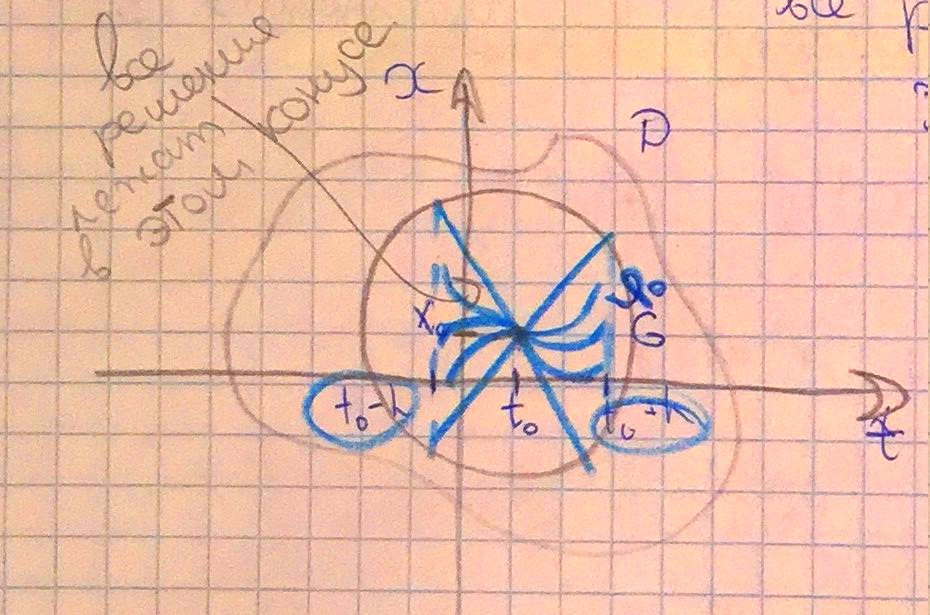
\includegraphics[width = 7cm]{proofPikar}

  $[t_0 - h, t_0 + h]$ отрезок на котором определены все решения

  Пусть $G$ выпуклая ограниченная область $(t_0, x_0) \in G$
  $$
  M = \sup_{(t,s) \in G} ||f(t,x)||
  $$
  $$
  ||f|| = |f_1| + |f_2| + \ldots + |f_n|
  $$
  $$
  K_n = \{(t,x) \in R \times R^n ~:~ ||x - x_0|| \le M|t-t_0| ~~
  t \in [t_0 - h, t_0 + h\}
  $$
  кроме того уменьшая $h$ можно считать что график $\varphi_0$ лежит
  $t \in [t_0 - h, t_0 + h] ~~ \varphi_0(t) \subset G$

  Докаже что график всех приближений лежат в области $G$ при $(t, \varphi_k(t))
  \in G$

  Допустим $\varphi_k(t)$ определена на $[t_0 - h, t_0 + h]$ и его графи лежит
  в области $G$ при $(t, \varphi_k(t)) \in G$
  $$
  \varphi_{k+1}(t) = x_0 + \int_{t_0}^t f(s, \varphi_k(s))ds ~
  \text{непрерывна}
  $$
  $\varphi_{k+1}(t)$ определа на $[t_0 - h, t_0 + h]$

  Расмотрим
  $$
  ||\varphi_{k+1}(t) - x_0|| = \left\Vert \int_{t_0}^t f(s, \varphi_k(s))ds
  \right\Vert \le
  $$
  $$
  \le \left| \int_{t_0}^t \left\Vert f(s, \varphi_k(s))\right\Vert ds \right|
  \le M\left| \int_{t_0}^t \right| = M|t-t_0|
  $$
  $(t, \varphi_{k+1}(t))$ удовлитворяет равенству определяющему конус

  $\varphi_k(t)$ поределны на одном и том же $[t_0 - h, t_0 + h]$ $(t,
  \varphi_k(t)) \in K_n \subset G$

  2) Докажем равномерную сходимость приближений на $[t_0 - h, t_0 + h]$

  $\{\varphi_k(t)\}$
  $$
  \varphi_0(t) + \sum_{k=0}^{\infty}(\varphi_{k+1}(t) - \varphi_k(t))
  $$
  $$
  S_n(t) = \varphi_0(t) + \sum_{k=0}^n (\varphi_{k+1}(t) - \varphi_k(t) =
  $$
  $$
  = \varphi_0(t) + \varphi_1(t) - \varphi_0(t) + \varphi_2(t) - \varphi_1(t),
  \ldots, + \varphi_{n+1}(t) - \varphi_n(t)) = \varphi_{n+1}(t)
  $$
  Из теоремы Вейерштрасса $\sum_{k=0}^{\infty} f_k(t) ~~ t \in T$ и
  $|f_k(t) \le b_k(t)$ и $\sum_{k=0}^{\infty} b_k(t)$ сходится тогда
  $\sum_{k=0}^{\infty} f_k(t)$ равномерно сходится

  Оценим норму
  $$
  ||\varphi_{k+1}(t) - \varphi_k(t)||
  $$
  $$
  k = 0 ~~ ||\varphi_1(t) - \varphi_0(t)||
  $$
  $$
  N = \sup_{t \in [t_0 - h, t_0 + h]} ||\varphi_1(t) - \varphi_0(t)||
  $$
  $$
  ||f(t, x) - f(t,y)|| \le \sup_{(t,x ) \in G} \left\Vert \frac{\partial f}{
  \partial x} \right\Vert ||x-y||
  $$
  $\frac{\partial f}{\partial x}$ непрерывная матрица Якоби $\Rightarrow$
  $\sup \frac{\partial f}{\partial x} = L = \const$

  значит получаем условие Липница
  $$
  ||f(t,x) - f(t,y)|| \le L||x-y||
  $$
  $$
  ||\varphi_2(t) - \varphi_1(t)|| = \left\Vert x_0 + \int_{t_0}^n
  f(s, \varphi_1(s))ds - x_0 - \int_{t_0}^t f(s, \varphi_0(s))ds \right\Vert =
  $$
  $$
  \left\Vert \int_{t_0}^n f(s, \varphi_1(s)) - f(s, \varphi_0(s))ds \right\Vert
  \le
  $$
  $$
  \le \left| \int_{t_0}^n ||f(s, \varphi_1(s)) - f(s, \varphi_0(s))||ds
  \right| \le
  $$
  $$
  \le \left| \int_{t_0}^n ||\varphi_1(s) - \varphi_0(s)||ds \right| \le
  LN|t-t_0| \le LND
  $$
  $$
  ||\varphi_3(t) - \varphi_2(t)|| = \left\Vert x_0 + \int_{t_0}^n
  f(s, \varphi_2(s))ds - x_0 - \int_{t_0}^t f(s, \varphi_1(s))ds \right\Vert =
  $$
  $$
  \left\Vert \int_{t_0}^n f(s, \varphi_2(s)) - f(s, \varphi_1(s))ds \right\Vert
  \le
  $$
  $$
  \le \left| \int_{t_0}^n ||f(s, \varphi_2(s)) - f(s, \varphi_1(s))||ds
  \right| \le
  $$
  $$
  \le \left| \int_{t_0}^n L||\varphi_2(s) - \varphi_1(s)||ds \right| \le
  $$
  $$
  \le L \left| \int_{t_0}^n LN|s-t_0|ds \right| = L^2 N \int_{t_0}^t
  |s-t_0|ds =
  $$
  $$
  \int_{t_0}^t |s - t_0| ds =
  \left\{
  \begin{array}{l}
  \int_{t_0}^t |s - t_0| ds, ~ t \ge t_0 \\
  \int_{t_0}^t |t_0 - s| ds, ~ t < t_0
  \end{array}
  \right. =
  \left\{
  \begin{array}{l}
    \frac{(s - t_0)^2}{2}|_{t_0}^t \\
    \frac{-(t_0 - s)^2}{2}|_{t_0}^t
  \end{array}
  \right. =
  \left\{
  \begin{array}{l}
    \frac{(t - t_0)^2}{2} \\
    \frac{-(t_0 - t)^2}{2}
  \end{array}
  \right.
  $$
  $$
  = L^2N\frac{|t - t_0|^2}{2}
  $$
  $$
  ||\varphi_3 - \varphi_2|| \le \frac{L^2N|t-t_0|^2}{2} ~ \Rightarrow ~
  ||\varphi_{k+1} - \varphi_k|| \le \frac{L^kN|t-t_0|^k}{k!}
  $$
  Докажем метадом мат индукции $k \to k+1$
  $$
  ||\varphi_{k+2} + \varphi_{k+1}(t)|| = \left\Vert x_0 + \int_{t_0}^t
  f(s, \varphi_{k+1}(s))ds - x_0 - \int_{t_0}^t
  f(s, \varphi_k(s))ds\right\Vert \le
  $$
  $$
  \le \ldots \le \left| \int_{t_0}^t L||\varphi_{k+1}(s) - \varphi_k(s)||ds
  \right| \le
  $$
  $$
  \le \frac{L^{k+1}N}{k!}\left| \int_{t_0}^t |s - t_0|^k ds \right| =
  \frac{L^{k+1}N}{(k+1)!}|t-t_0|^{k+1}
  $$
  $\Rightarrow$ оценка справидлива $\forall k \in N$
  $$
  \frac{L^k N D^k}{k!} = b_k ~ \Rightarrow ||\varphi_0(t)|| +
  \sum_{k=0}^{\infty} \frac{L^kN D^k}{k!}
  $$
  По признаку Даламбера
  $$
  \frac{b_{k+1}}{b_k} = \frac{L^{k+1}ND^k+1}{(k+1)!} \frac{k!}{L^K N D^k} =
  \frac{LD}{k+1} \to 0 ~ k \to \infty
  $$
  $\Rightarrow$ $||\varphi_0(t)|| + \sum_{k=0}^{\infty} \frac{L^kND^k}{k!}$
  сходится

  Значит по признаку Вейерштраса функциональный ряд
  $$
  \varphi_0(t) + \sum_{k=0}^{\infty} (\varphi_{k+1}(t) - \varphi_k(t)) ~
  \text{сходится равномерно на} [t_0 - h, t_0 + h]
  $$
  $\varphi_k(t) \rightrightarrows \varphi(t)$
  $$
  \varphi_0(t) + \sum_{k=0}^{\infty} (\varphi_{k+1}(t) - \varphi_k(t)) =
  \varphi(t)
  $$
  $$
  \varphi_{k+1} = x_0 \int_{t_0}^t f(s, \varphi_k(s))ds
  $$
  $$
  \downarrow ~~~~~~~~ \downarrow ~~~~~~~~ \downarrow
  $$
  $$
  \varphi = x_0 \int_{t_0}^t f(s, \varphi(s))ds
  $$
  Покажем что
  $$
  \int_{t_0}^t f(s, \varphi_k(s))ds \to \int_{t_0}^t f(s, \varphi(s))ds ~
  k \to \infty
  $$
  $$
  \left\Vert \int_{t_0}^t f(s, \varphi_k(s))ds - \int_{t_0}^t
  f(s, \varphi(s))ds \right\Vert \le
  $$
  $$
  \le \left| \int_{t_0}^t ||f(s, \varphi_k(s)) -
  f(s, \varphi(s))||ds \right| \le
  $$
  $$
  \le L \left|\int_{t_0}^t ||\varphi_k(s)) - \varphi(s))||ds \right| \le
  $$
  $$
  \le L\max_{s \in [t_0, t]} ||\varphi_k(s)) - \varphi(s))|| \cdot |t-t_0|
  \to 0
  $$
  $||\varphi_k(s)) - \varphi(s))|| \to 0 ~~ k \to 0$

  Переходя к формуле пределов $\varphi(t)$ удовлитворяет интегральному
  уравнению

  По Лемме $\varphi(t)$ является решением задачи Коши

  3) Единственость $\varphi(t)$

  Пусть есть другое решение $\psi(t)$
  $$
  N_1 = \max_{t\in [t_0-h, t_0+h]} ||\varphi(t) - \psi(t)||
  $$
  $$
  \varphi(t) = x_0 + \int_{t_0}^t f(s, \varphi(s))ds
  $$
  $$
  \psi(t) = x_0 + \int_{t_0}^t f(s, \psi(s))ds
  $$
  $$
  ||\varphi(t) - \psi(t)|| = \left\Vert \int_{t_0}^t (f(s, \varphi(s) -
  f(s, \psi(s)))ds \right\Vert \le
  $$
  $$
  \le \left| \int_{t_0}^t ||f(s, \varphi(s)) + f(s, \psi(s))||ds \right| \le
  $$
  $$
  \le L \left| \int_{t_0}^t ||\varphi(s) - \psi(s)||ds \right| \le
  $$
  $$
  \le L \left| \int_{t_0}^t N_1 L |s-t_0|ds \right| = \frac{L^2N}{2}|t-t_0|^2
  \le N_1 L |t-t_0|
  $$
  $$
  ||\varphi(t) - \psi(t)|| = \frac{L^kN_1|t-t_0|^k}{k!} \to 0 ~ \Rightarrow ~
  \varphi(t) \equiv \psi(t)
  $$
\end{proof}